\section{Конструкторская часть}

В данном разделе рассмотрено проектирование базы данных и системы создания нормативных документов рабочей программы дисциплины и фонда оценочных средств, являющейся частью системы управления обучением. 

\subsection{Проектирование системы}

Проектируемая система состоит из БД компонентов нормативных документов и пользовательского приложения для их добавления, редактирования и удаления, а также создания РПД и ФОС. Диаграмма последовательностей представлена на рисунке \ref{img:seq}.

\begin{figure}[h!]
	\begin{center}
		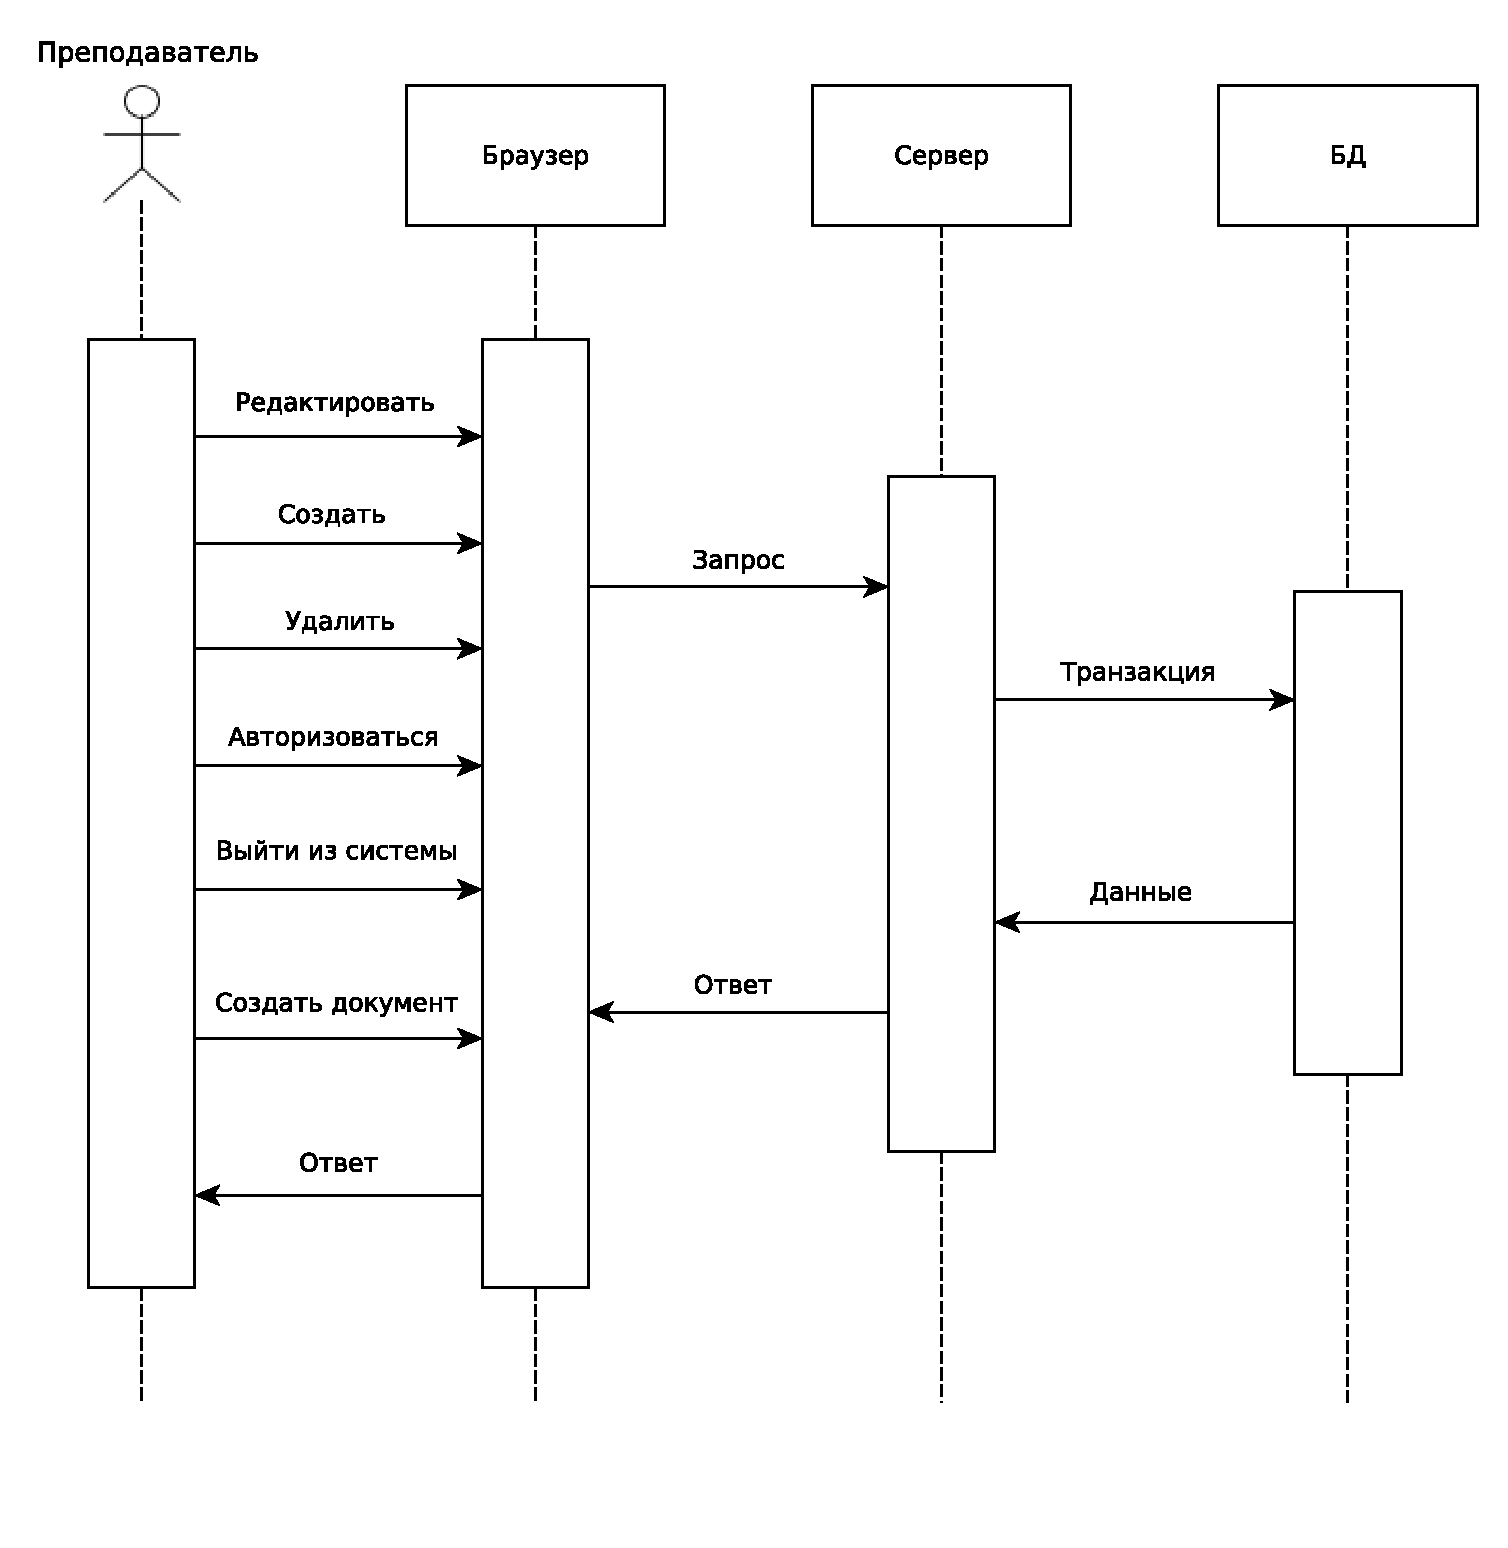
\includegraphics[scale=0.4666]{inc/img/sequence}
	\end{center}
	\captionsetup{justification=centering}
	\caption{Диаграмма последовательностей}
	\label{img:seq}
\end{figure}

\clearpage

\noindent\textbf{Роли пользователей}

В приложении определены две основные роли: 
\begin{enumerate}
	\item преподаватель -- работает с компонентами документов, хранящимися в базе данных, и составляет на их основе нормативные документы;
	\item администратор -- осуществляет управление системой.
\end{enumerate}
Схема распределения ролей представлена на рисунке \ref{img:usecase}.

\begin{figure}[h!]
	\begin{center}
		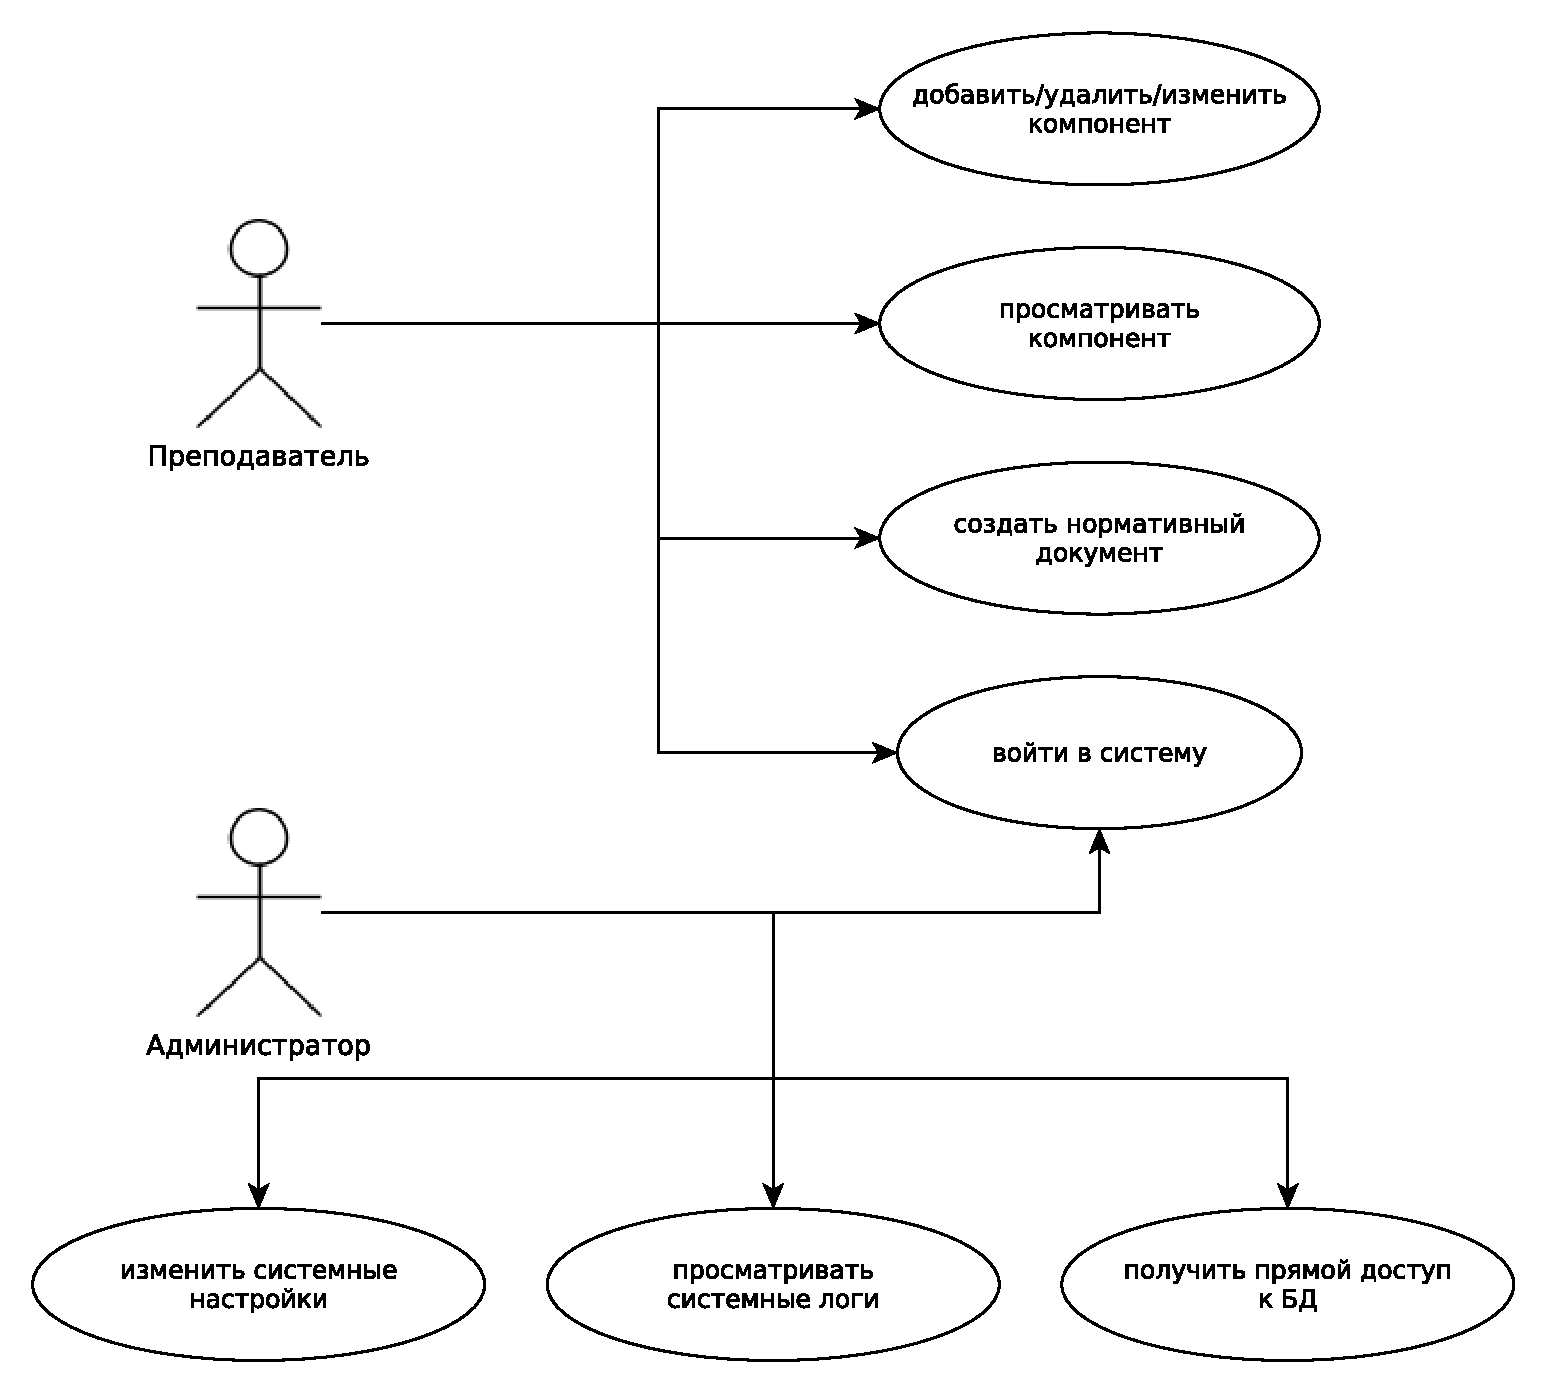
\includegraphics[scale=0.4]{inc/img/use_case}
	\end{center}
	\captionsetup{justification=centering}
	\caption{Роли пользователей в системе}
	\label{img:usecase}
\end{figure}

\noindent\textbf{Диаграмма функционирования системы}

Верхнеуровневая диаграмма представлена на рисунке \ref{img:idef0}, процесс составления документа представлен на рисунке \ref{img:idef0_2}. На вход система получает данные о компонентах нормативного документа, запрашивает их из базы данных, обрабатывает согласно структуре нормативного документа и на выходе формирует нормативный документ.

\clearpage

\begin{figure}[h!]
	\begin{center}
		\includegraphics[scale=0.22666]{inc/img/idef0.png}
	\end{center}
	\captionsetup{justification=centering}
	\caption{Верхнеуровневая диаграмма приложения}
	\label{img:idef0}
\end{figure}

\begin{figure}[h!]
	\begin{center}
		\includegraphics[scale=0.22666]{inc/img/idef0_2.png}
	\end{center}
	\captionsetup{justification=centering}
	\caption{Процесс составления документа}
	\label{img:idef0_2}
\end{figure}


\subsubsection{Проектирование базы данных}

Модель вида <<сущность-связь>> \cite{er-chen} представлена на рисунке \ref{img:er}.

\clearpage

\begin{figure}[h!]
	\begin{center}
		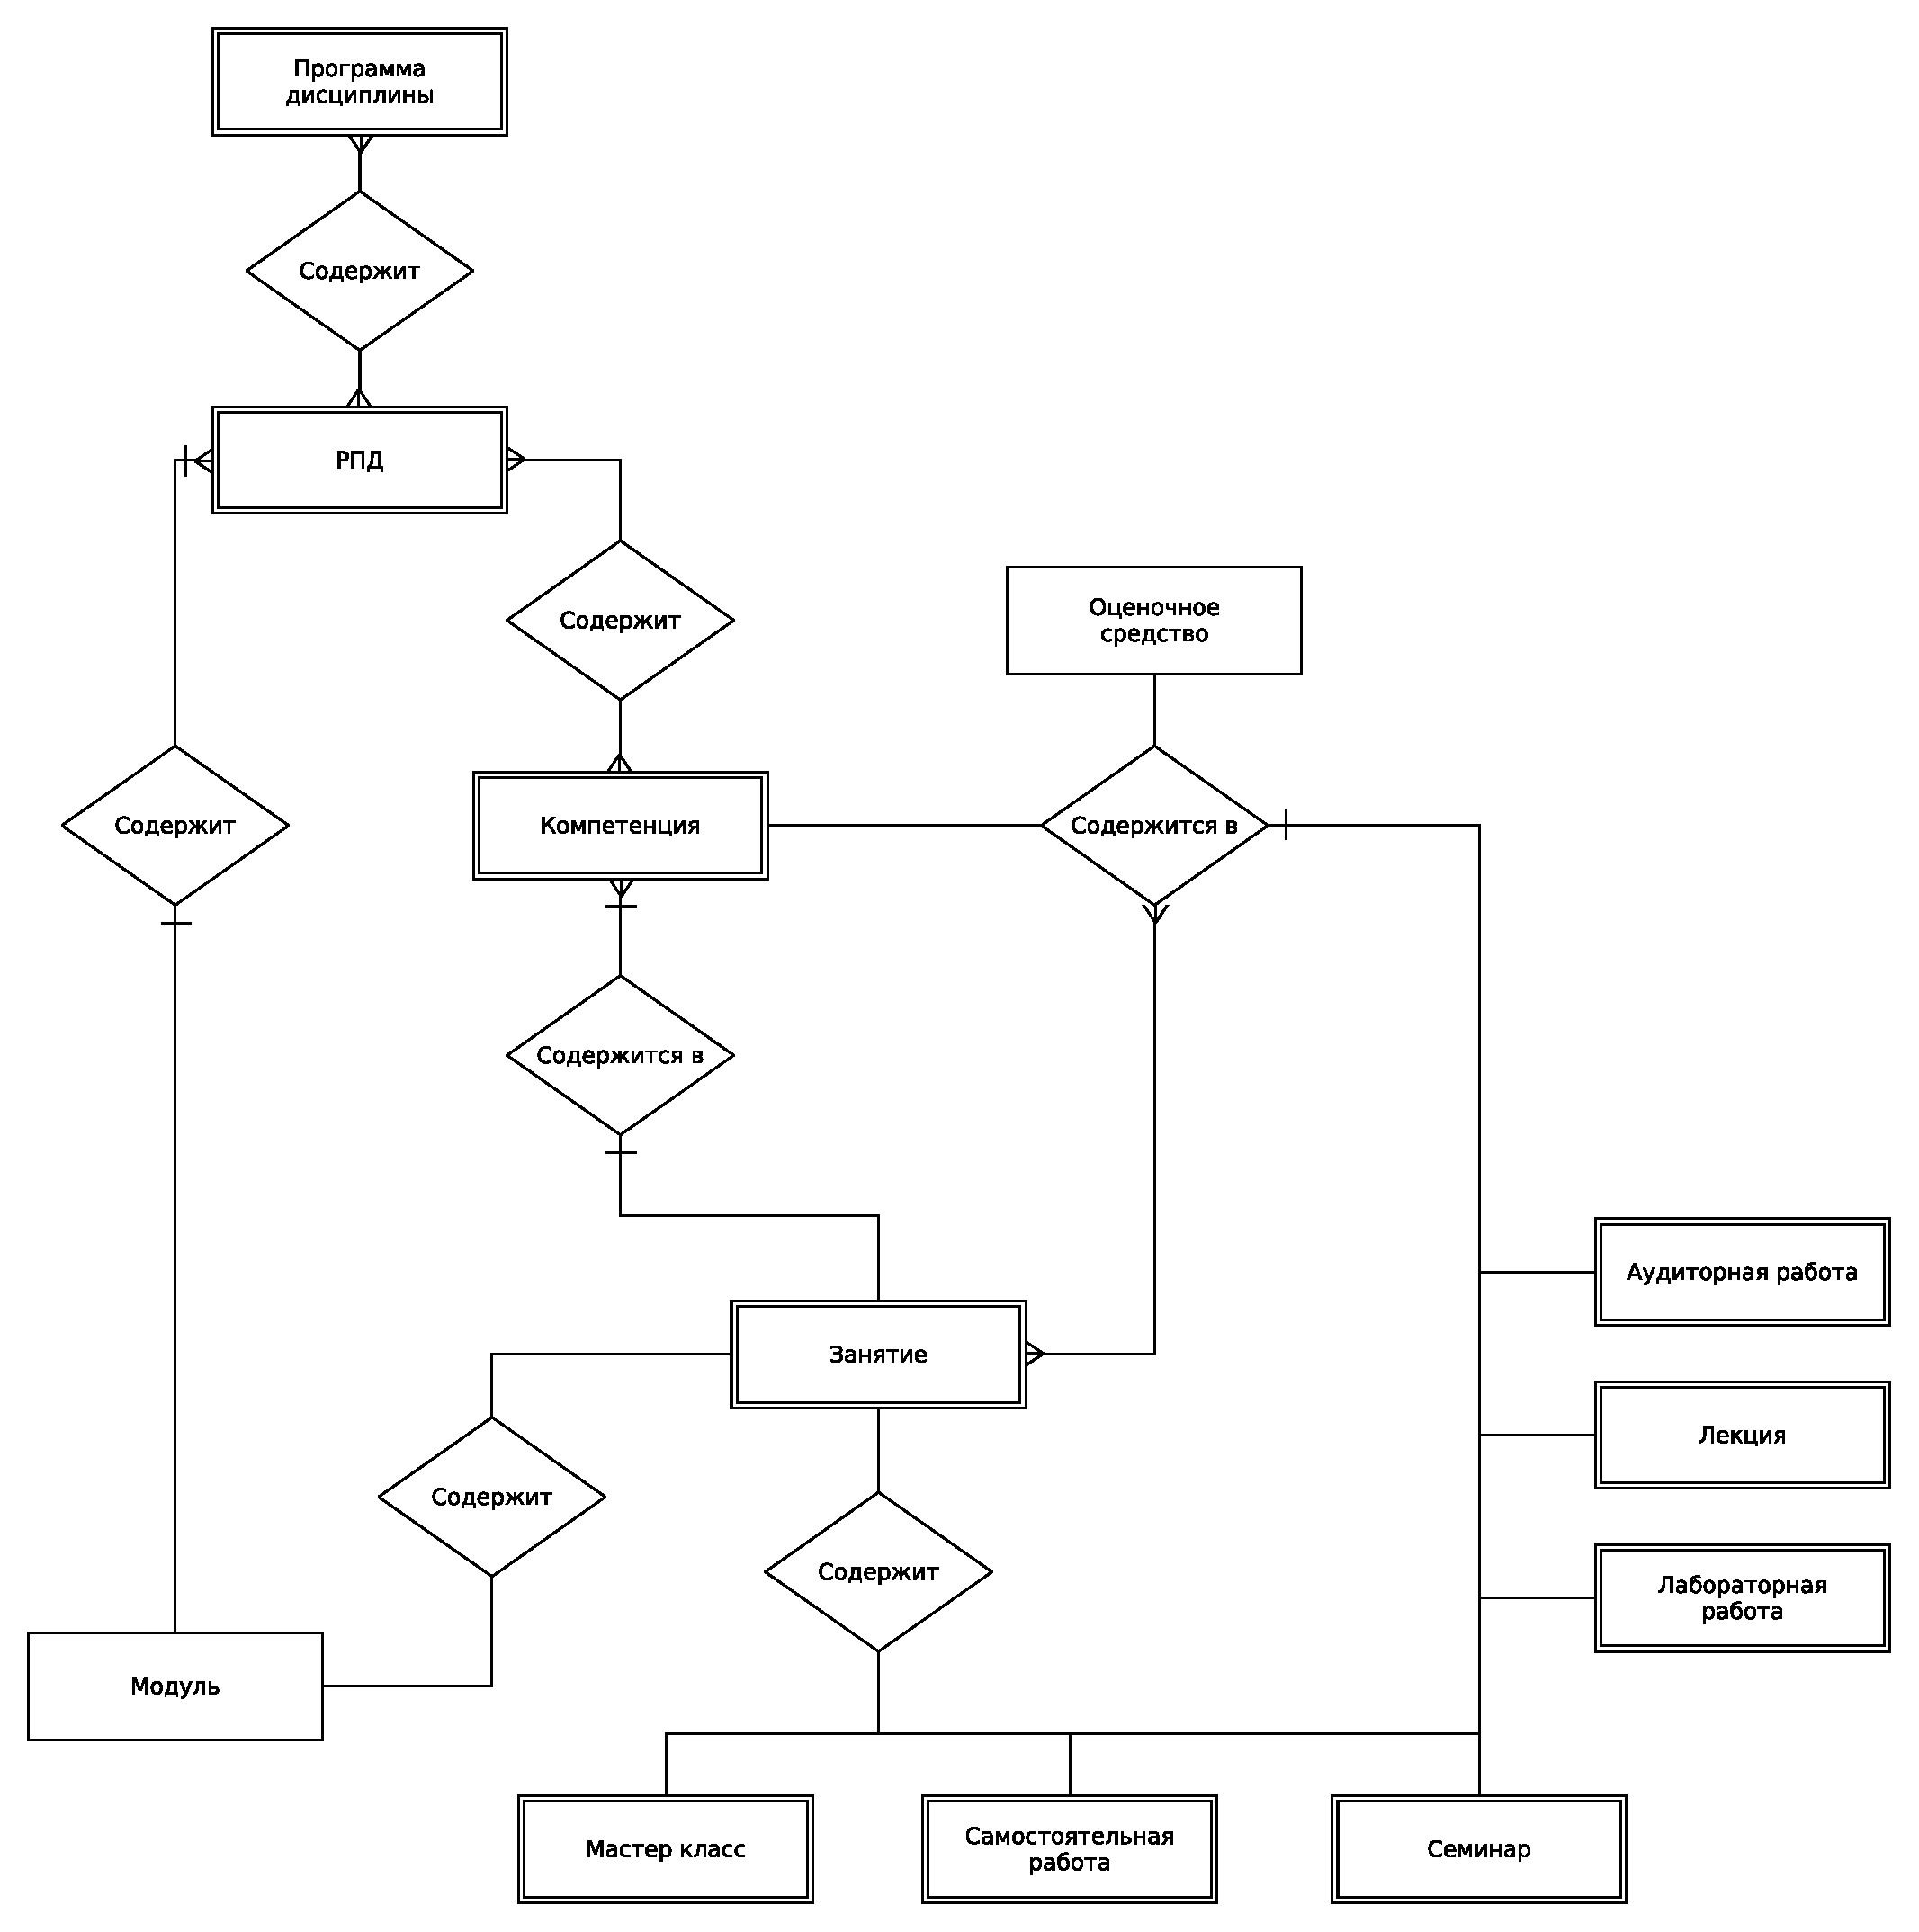
\includegraphics[scale=0.47]{inc/img/er.pdf}
	\end{center}
	\captionsetup{justification=centering}
	\caption{Модель <<сущность-связь>> в нотации Чена}
	\label{img:er}
\end{figure}

\noindent\textbf{Описание сущностей модели}

Программа дисциплины имеет следующие атрибуты:
\begin{itemize}
	\item название;
	\item описание;
	\item РПД.
\end{itemize}

\clearpage

РПД имеет следующие атрибуты:
\begin{itemize}
	\item название;
	\item код ФГОС;
	\item содержание;
	\item виды учебных занятий;
	\item компетенции;
	\item модули;
	\item результат обучения;
	\item материалы дисциплины;
\end{itemize}


Модуль имеет следующие атрибуты:
\begin{itemize}
	\item занятия;
	\item компетенции;
	\item оценочное средство;
	\item имя;
	\item количество часов для каждого типа работы;
	\item номер семестра;
\end{itemize}


Компетенция имеет следующие атрибуты:
\begin{itemize}
	\item имя;
	\item код;
	\item формулировка;
	\item тип;
	\item категория;
	\item этапы формирования;
	\item оценочное средство.
\end{itemize}

\clearpage

Занятие имеет следующие атрибуты:
\begin{itemize}
	\item имя;
	\item количество часов;
	\item компетенция;
	\item оценочное средство;
	\item тип занятия:
	\begin{itemize}
		\item мастер класс;
		\item самостоятельная работа;
		\item семинар;
		\item лабораторная работа;
		\item лекция;
		\item аудиторная работа.
	\end{itemize}
\end{itemize}

Мастер класс, самостоятельная работа, семинар, лабораторная работа, лекция и аудиторная работа имеют следующие атрибуты:
\begin{itemize}
	\item название;
	\item количество часов;
	\item тема;
	\item вид работы;
	\item оценочное средство.
\end{itemize}
